\documentclass{article}
\RequirePackage{amssymb}
\RequirePackage{amsmath}
\usepackage{graphicx}
\usepackage[latin1]{inputenc}

\title{Esercizio 2 di riepilogo}
\author{Davide Angelocola}

\begin{document}
\maketitle

\section{Testo del problema}

Sia

$$
P = \begin{pmatrix}
1 & 0 & 0 & 0 & 0 & 0 \cr 
\frac{1}{4} & \frac{1}{2} & \frac{1}{4} & 0 & 0 & 0 \cr 
0 & \frac{1}{5} & \frac{2}{5} & \frac{1}{5} & 0 & \frac{1}{5} \cr 
0 & 0 & 0 & \frac{1}{6} & \frac{1}{3} & \frac{1}{2} \cr 
0 & 0 & 0 & \frac{1}{2} & 0 & \frac{1}{2} \cr 
0 & 0 & 0 & \frac{1}{4} & 0 & \frac{3}{4} \cr 
\end{pmatrix}
$$

matrice di transizione su $S = \{ 1, 2, 3, 4, 5, 6 \}$.

\begin{itemize}
    \item i) determinare il carattere degli stati
    \item ii) Dimostrare che muovendosi dallo stato 4 con la dinamica descritta da $P$ la probabilit� di raggiungere lo stato 6 in un tempo finito � almeno $\frac{3}{4}$
    \item iii) Calcolare la probabilit� di raggiungere lo stato 1 partendo dallo stato 2 in un tempo finito, $p_{2 1}$ e dare un'interpretazione probabilistica del numero $1 - p_{2 1}$.
\end{itemize}

\section{i) Carattere degli stati}

Disegnamo il grafo delle transizioni:

\begin{figure}[h]
\centering
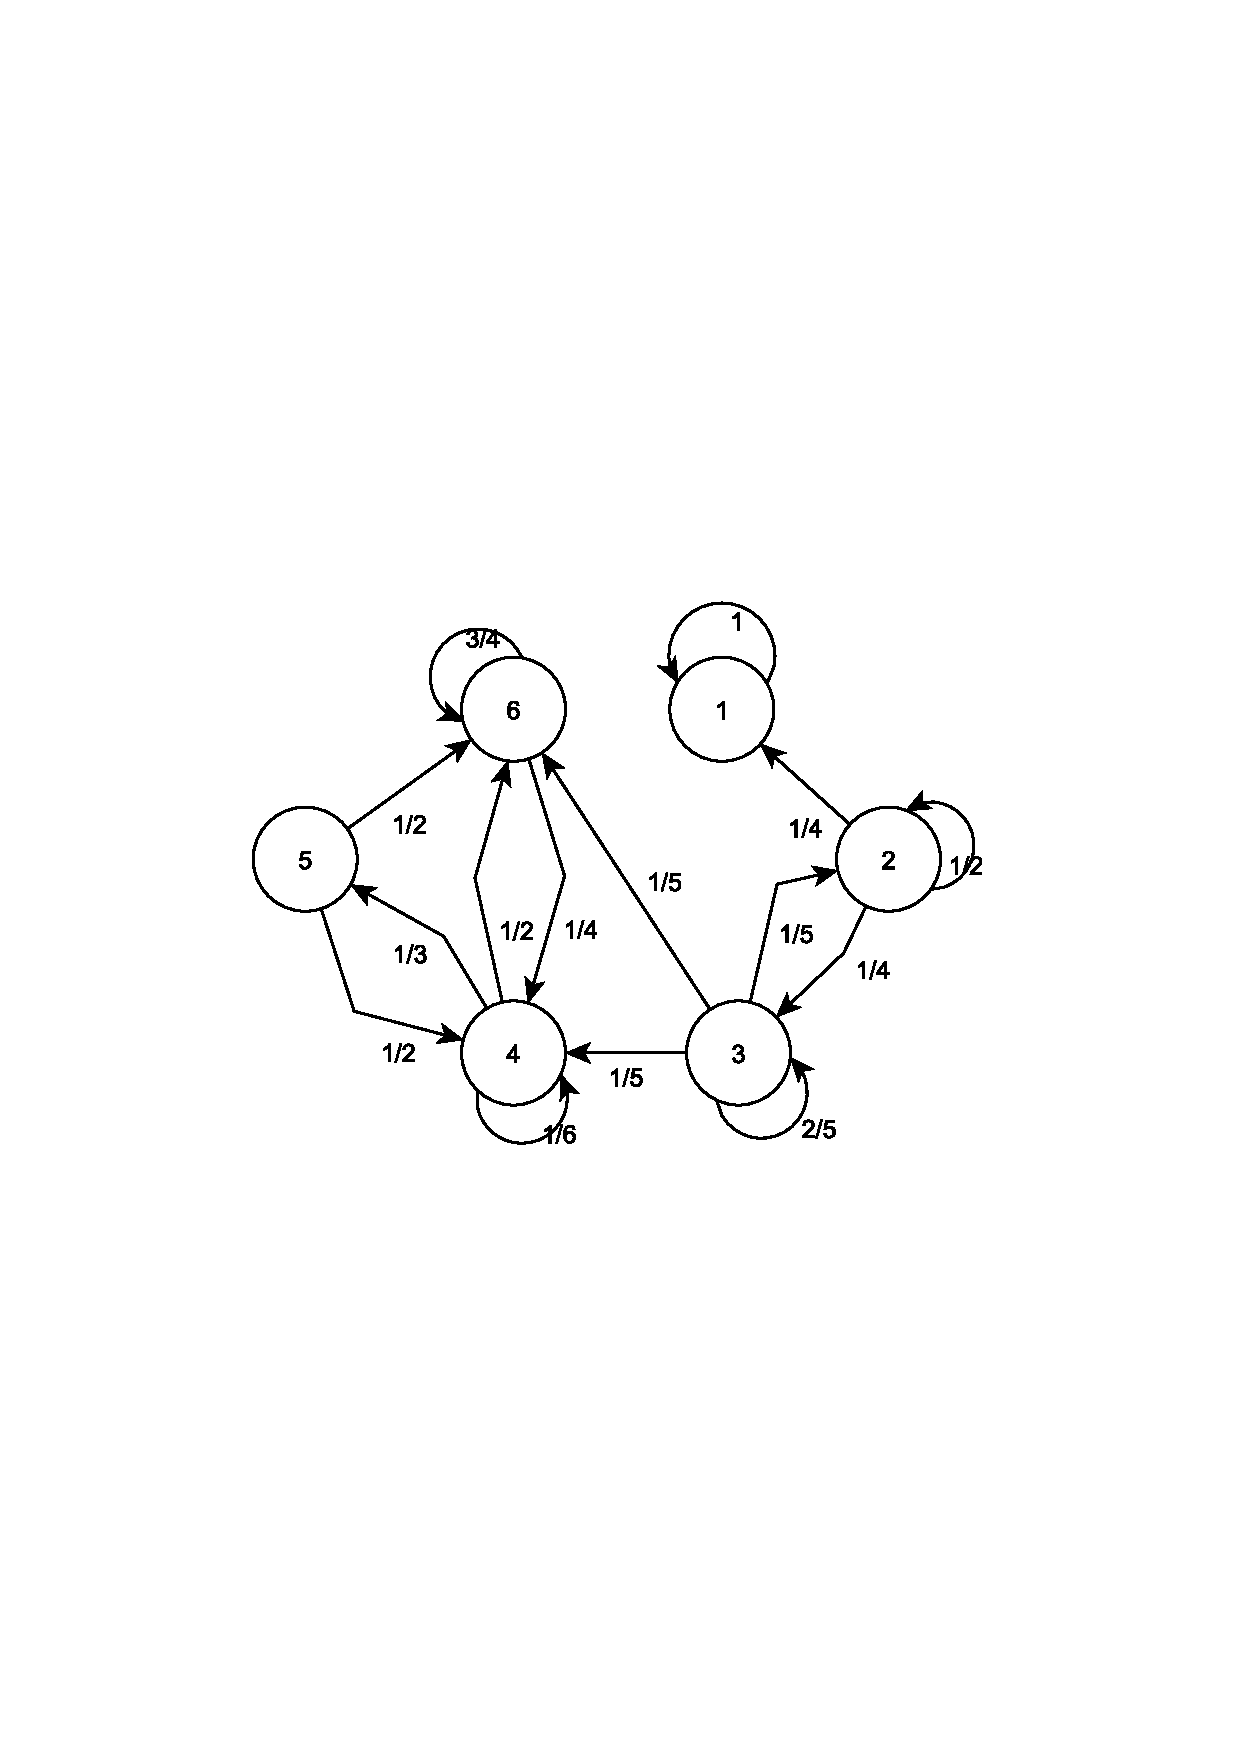
\includegraphics{cp_ex2_fig1.pdf}
\caption{}
\label{fig:}
\end{figure}

\begin{enumerate}
    \item � uno stato assorbente
    \item � uno stato transiente perch� comunica con 1 ma non � ricambiato
    \item � anch'esso transiente perch� comunica sia con 4 sia con 6 ma non � ricambiato
    \item forma, insieme agli stati 5 e 6, una classe irriducibile \footnote{cosa sono gli stati persistenti positivi?}
    \item forma, insieme agli stati 4 e 6, una classe irriducibile
    \item forma, insieme agli stati 4 e 5, una classe irriducibile
\end{enumerate}

\section{ii)}

Considerando la classe irriducibile trasformata in modo tale che lo stato 6 sia assorbente:

\begin{figure}[h]
\centering
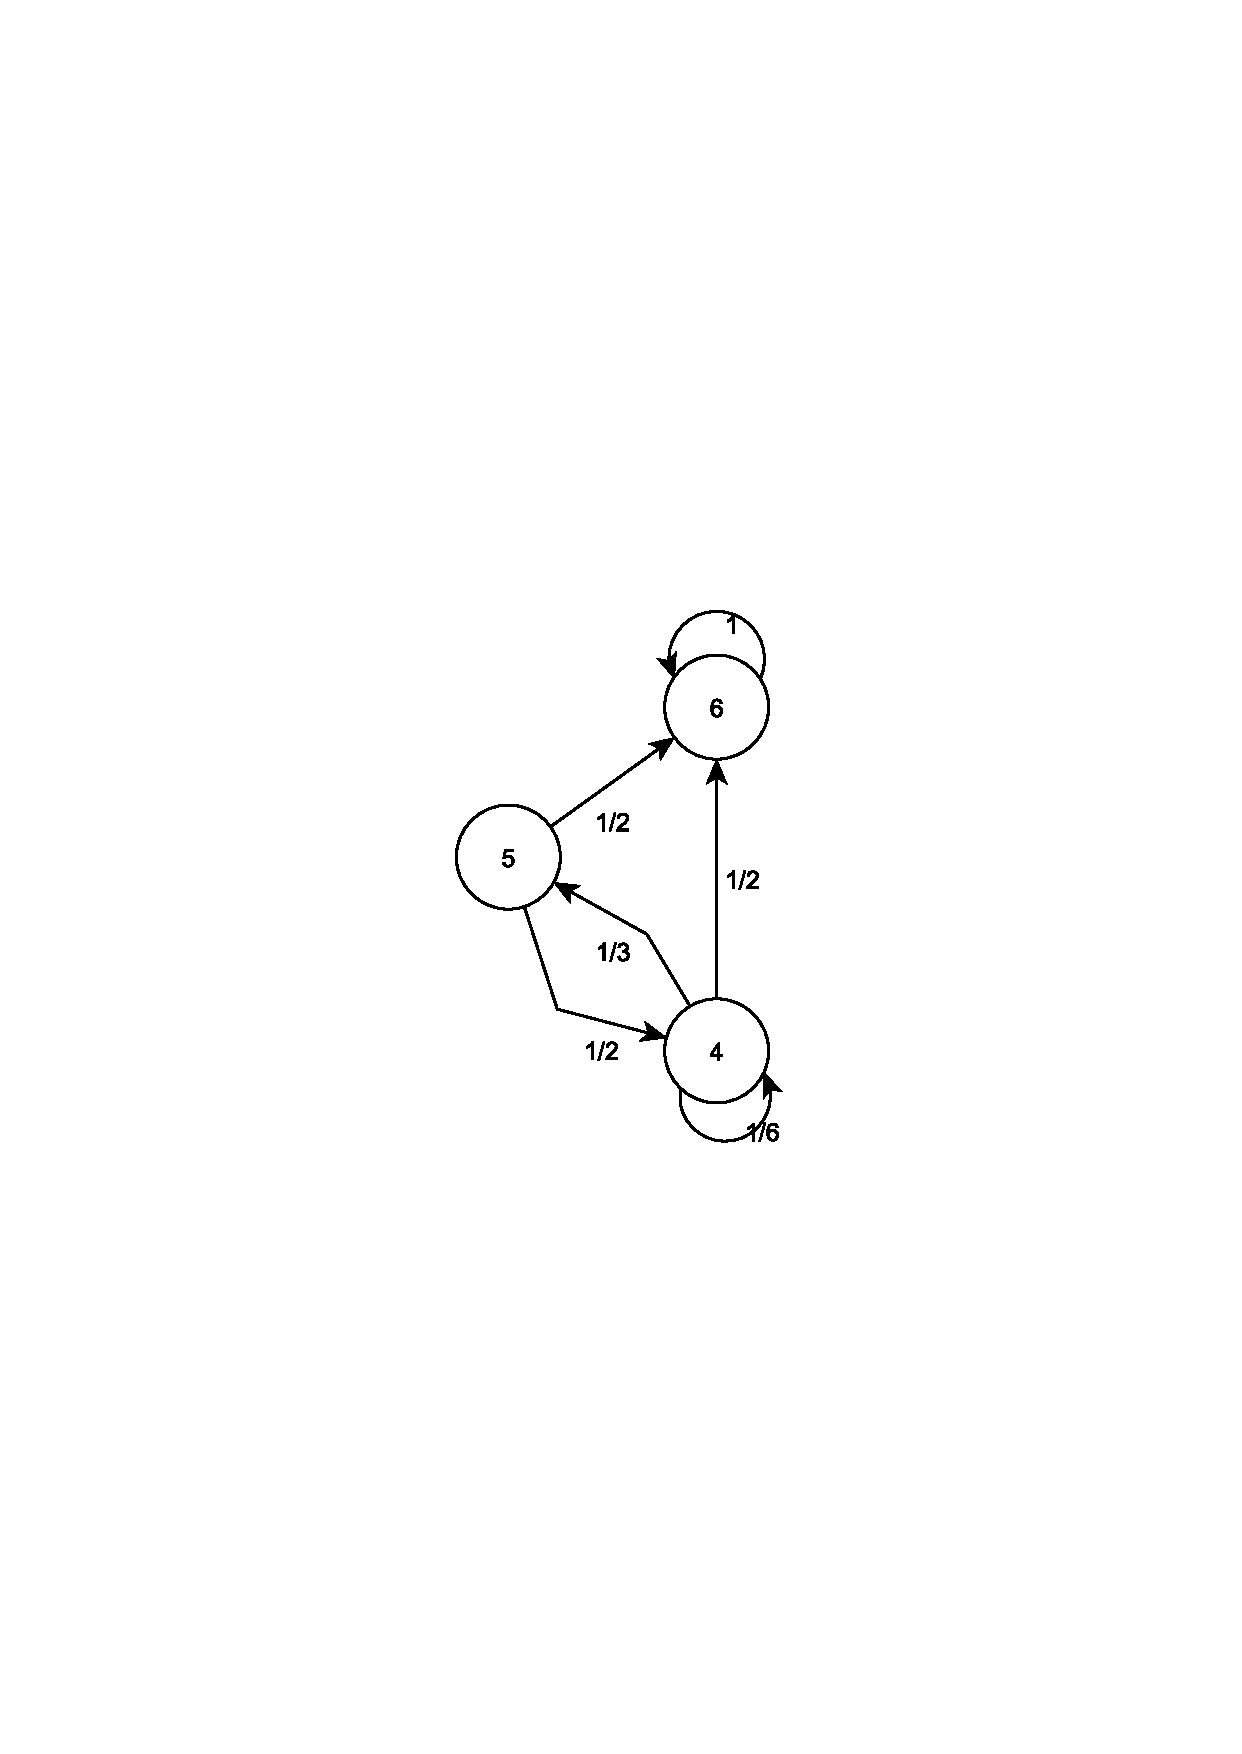
\includegraphics{cp_ex2_fig2.pdf}
\caption{}
\label{fig:}
\end{figure}

Possiamo ora calcolare la probabilit� di essere assorbiti in un tempo finito nello stato 6 a partire da 4 applicando la seguente formula:

\begin{equation} 
x_i = \sum_{j \in S \backslash T}{p_{i j}} + \sum_{j \in T}{p_{i j}x_j}, \forall i \in T
 \label{eq:1}
\end{equation}

con $T = \{ 4, 6\}$ si ottiene il seguente sistema:

$$ x_4 = \frac{1}{2} + \frac{1}{3}x_5$$
$$ x_5 = \frac{1}{2} + \frac{1}{4}x_4$$

sostituendo $x_5$ nella prima si ottiene:

$$x_4 = \frac{1}{2} + \frac{1}{3}(\frac{1}{2} + \frac{1}{2}x_4) = \frac{4}{5}$$

e:

$$x_5 = \frac{1}{2} + \frac{1}{2}\frac{4}{5} = \frac{9}{10}$$

Applicando ora la:

$$
P(\tau_6 < +\inf) = \sum_{j \in S}{\lambda_{j}^{\{6\}}p}  
$$

possiamo calcolare la probabilit� di essere assorbiti nello stato 6 partendo dallo stato 4:

$$ 
P(\tau_6 < +\inf) = \frac{4}{5} \frac{1}{2} + \frac{9}{10}\frac{1}{2} = \frac{17}{20}   
$$

che risulta essere maggiore di $\frac{3}{4}$, verificando quanto richiesto.

\section{iii)}

Essendo lo stato 1 assorbente per calcolare la probabilit� di raggiungerlo in tempo finito a partire da $2$ occorre calcolare $\lambda_2^{\{1\}}$ usando:
 
\begin{equation} 
x_i = \sum_{j \in S \backslash T}{p_{i j}} + \sum_{j \in T}{p_{i j}x_j}, \forall i \in T
 \label{eq:1}
\end{equation}

Risolvendo il sistema:

$$x_2=\frac{1}{4} + \frac{1}{2}x_2 + \frac{1}{4}x_3$$
$$x_3=\frac{1}{5}x_2 + \frac{1}{4}x_3$$

si ottiene:

$$x_2 = \frac{3}{5}$$ 
$$x_3 = \frac{1}{5}$$

La quantit� $1 - \rho_{21}$ � la probabilit� di non essere assorbiti in $1$ in un tempo finito. Per la natura di questa catena ci� equivale ad essere assorbiti nella classe irriducibile ${4, 5, 6}$. Poich� gli stati transienti sono in numero finito intuitivamente si deve "cadere" o nella classe ${1}$ o nella classe ${4, 5, 6}$. 

\end{document}
